\documentclass[8pt,xcolor=dvipsnames]{beamer}
\usepackage[latin1]{inputenc}

\usetheme[height=7mm]{Berlin}
\usecolortheme[named=Brown]{structure} 


\usepackage{time}       % date and time
\usepackage{graphicx}
\usepackage[T1]{fontenc}    % european characters
%\usepackage{courier}
\usepackage{animate}
\usepackage{multirow}
\usepackage{natbib}
\usepackage{amssymb,amsmath}  % use mathematical symbols
\usepackage{bookman}                  % use palatino as the default font
\setbeamercovered{transparent}
%\newcommand{figpath}{/Users/bhargavvaidya/MyProject/work/Leeds_Uni/SiOJets_New/PAPER/PFIGS}

\title[SiO Outflows]{Modeling SiO Emission from early outflows}
\subtitle{Extremely High Velocity Component [ EHV ]}
\author[Bhargav Vaidya]{\textcolor{blue}{Bhargav Vaidya}\inst{1} \and  Thomas
  Douglas\inst{1} \and Paola Caselli\inst{1}}\institute[]{\inst{1}School of Physics and
  Astronomy, University of Leeds, Leeds.}
\date[2013]{Pizza Meeting}
\titlegraphic{\vskip30pt \hskip215pt
\includegraphics[width=0.3\textwidth]{/Users/bhargavvaidya/MyProject/work/Leeds_Uni/SiOJets_New/PAPER/PFIGS/Leeds-logo.jpg}}

\begin{document}

%\begin{frame}
%\titlepage
%\end{frame}

\begin{frame}[l]
\frametitle{HH212 : A classic young jet.}
\begin{tabular}{ccc}
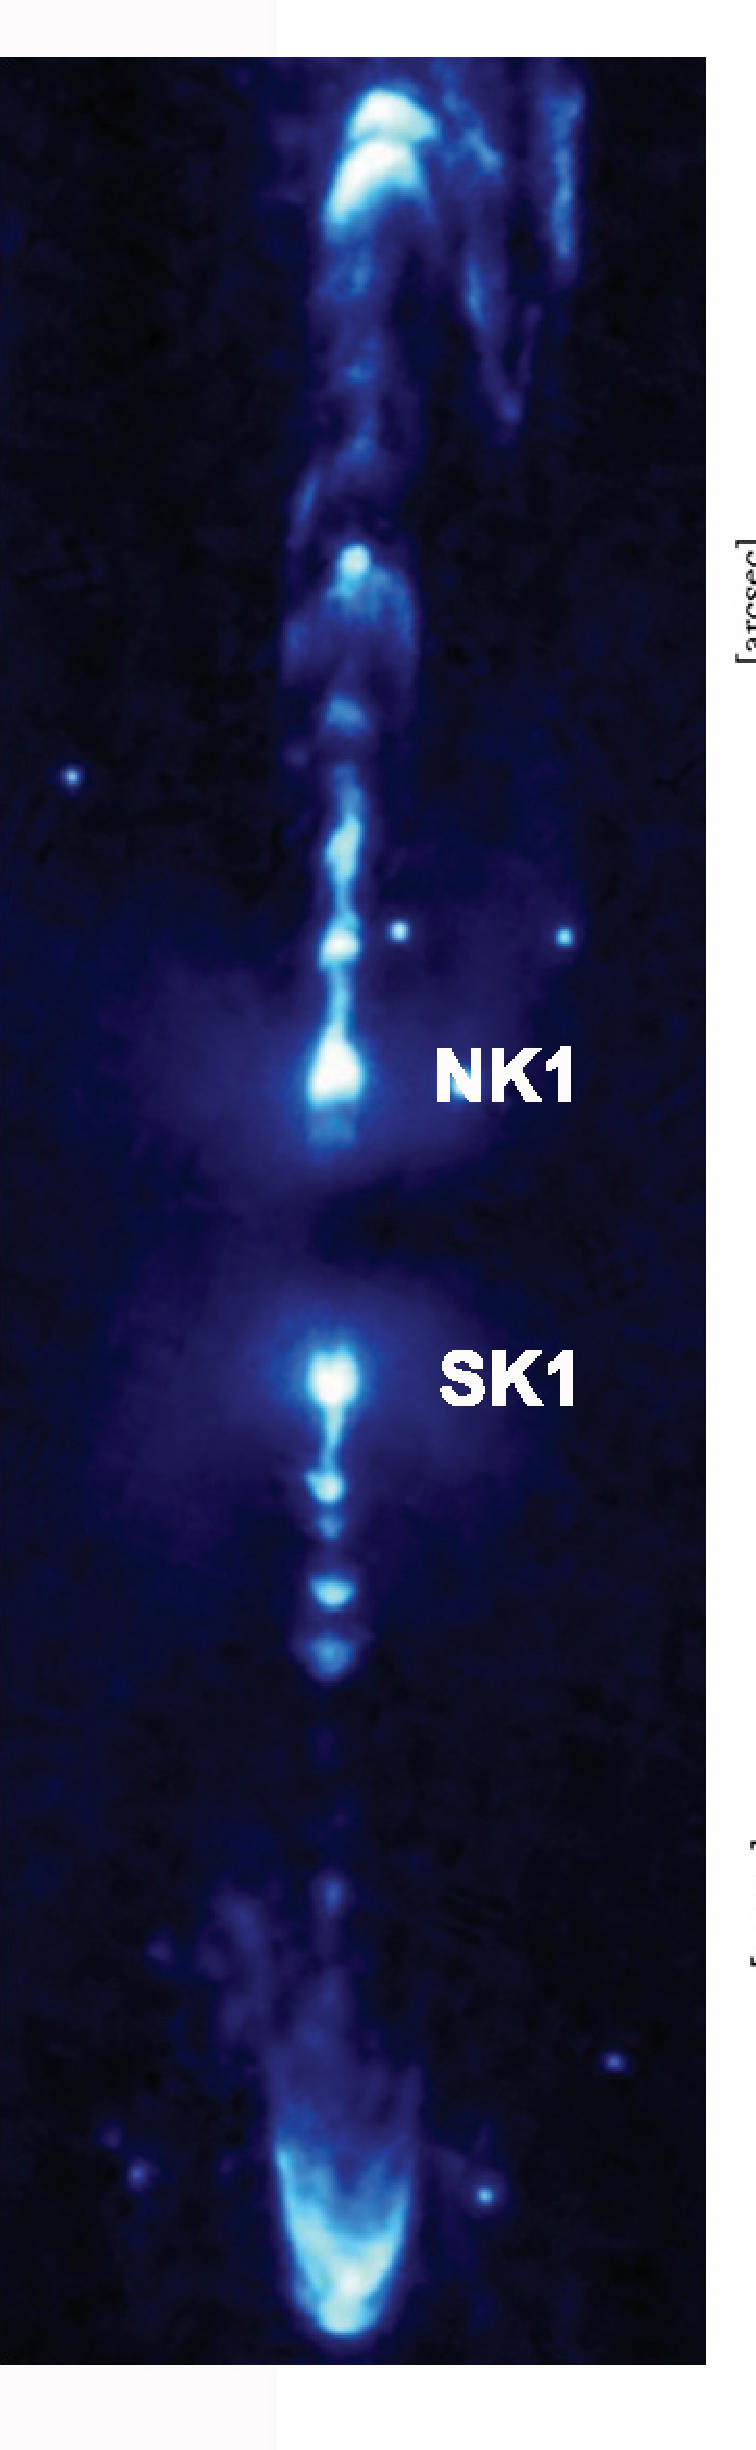
\includegraphics[scale=0.13]{hh212_best.pdf} & 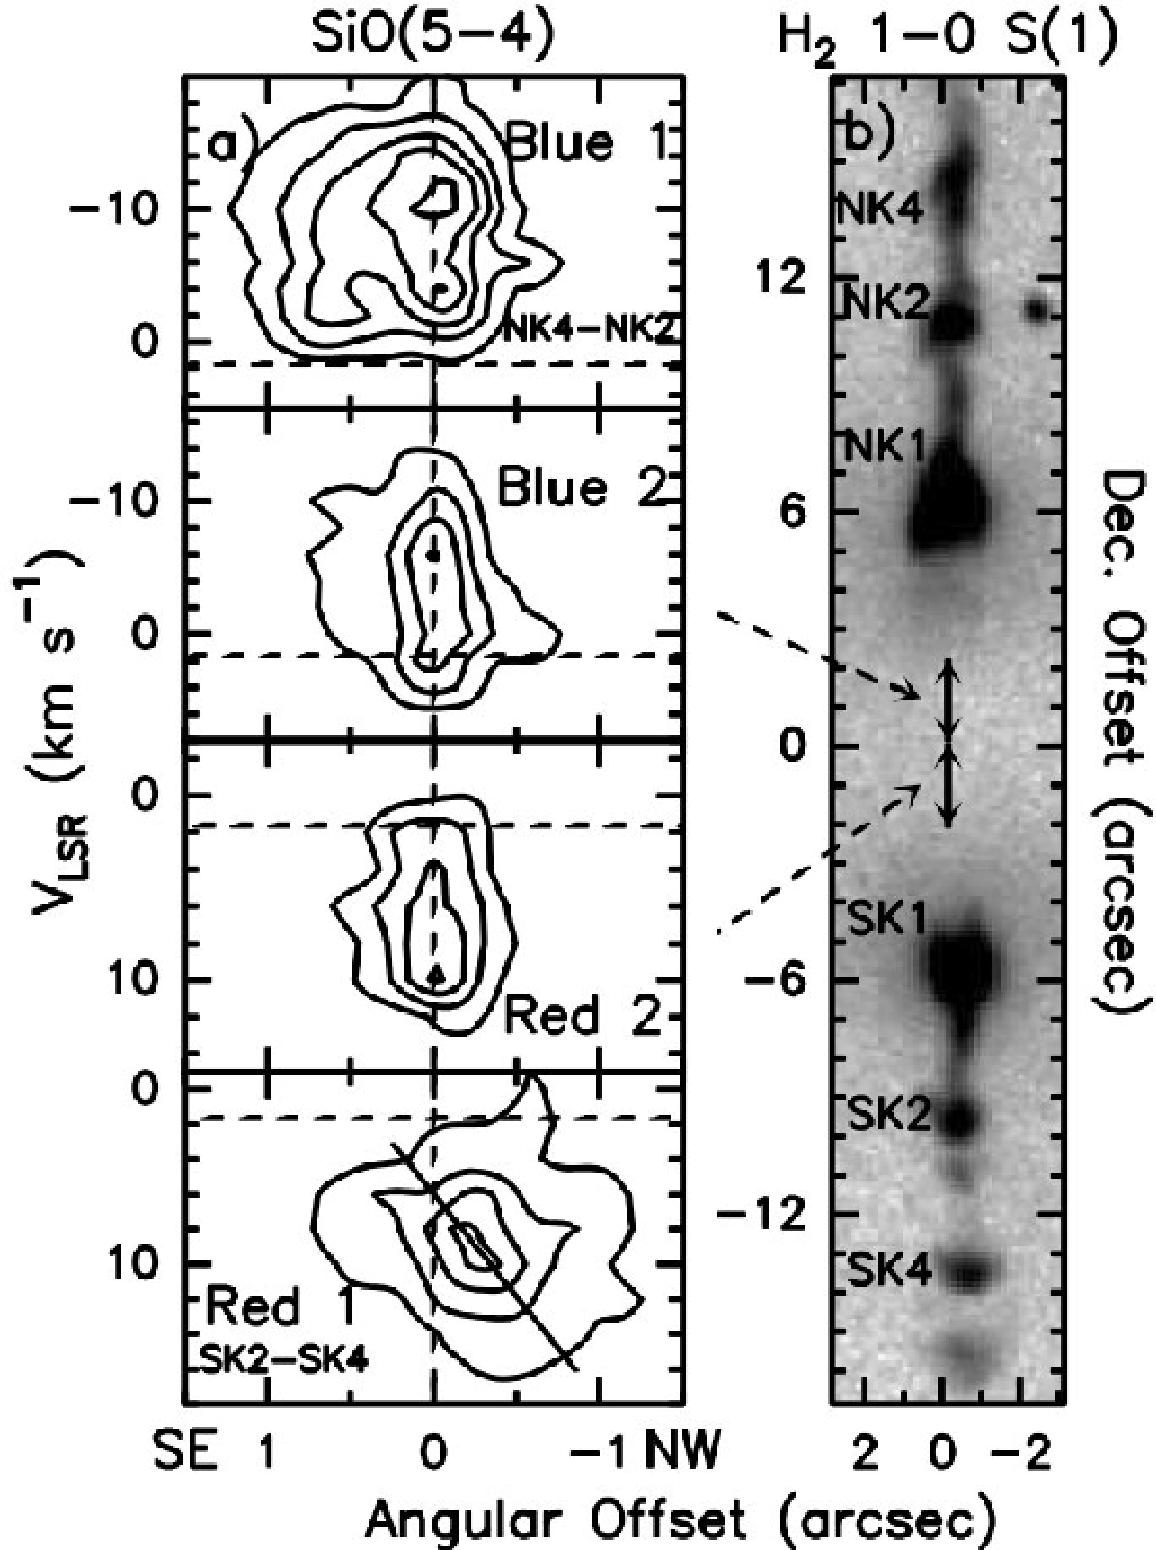
\includegraphics[scale=0.18]{codella_hh212_f3.pdf} & 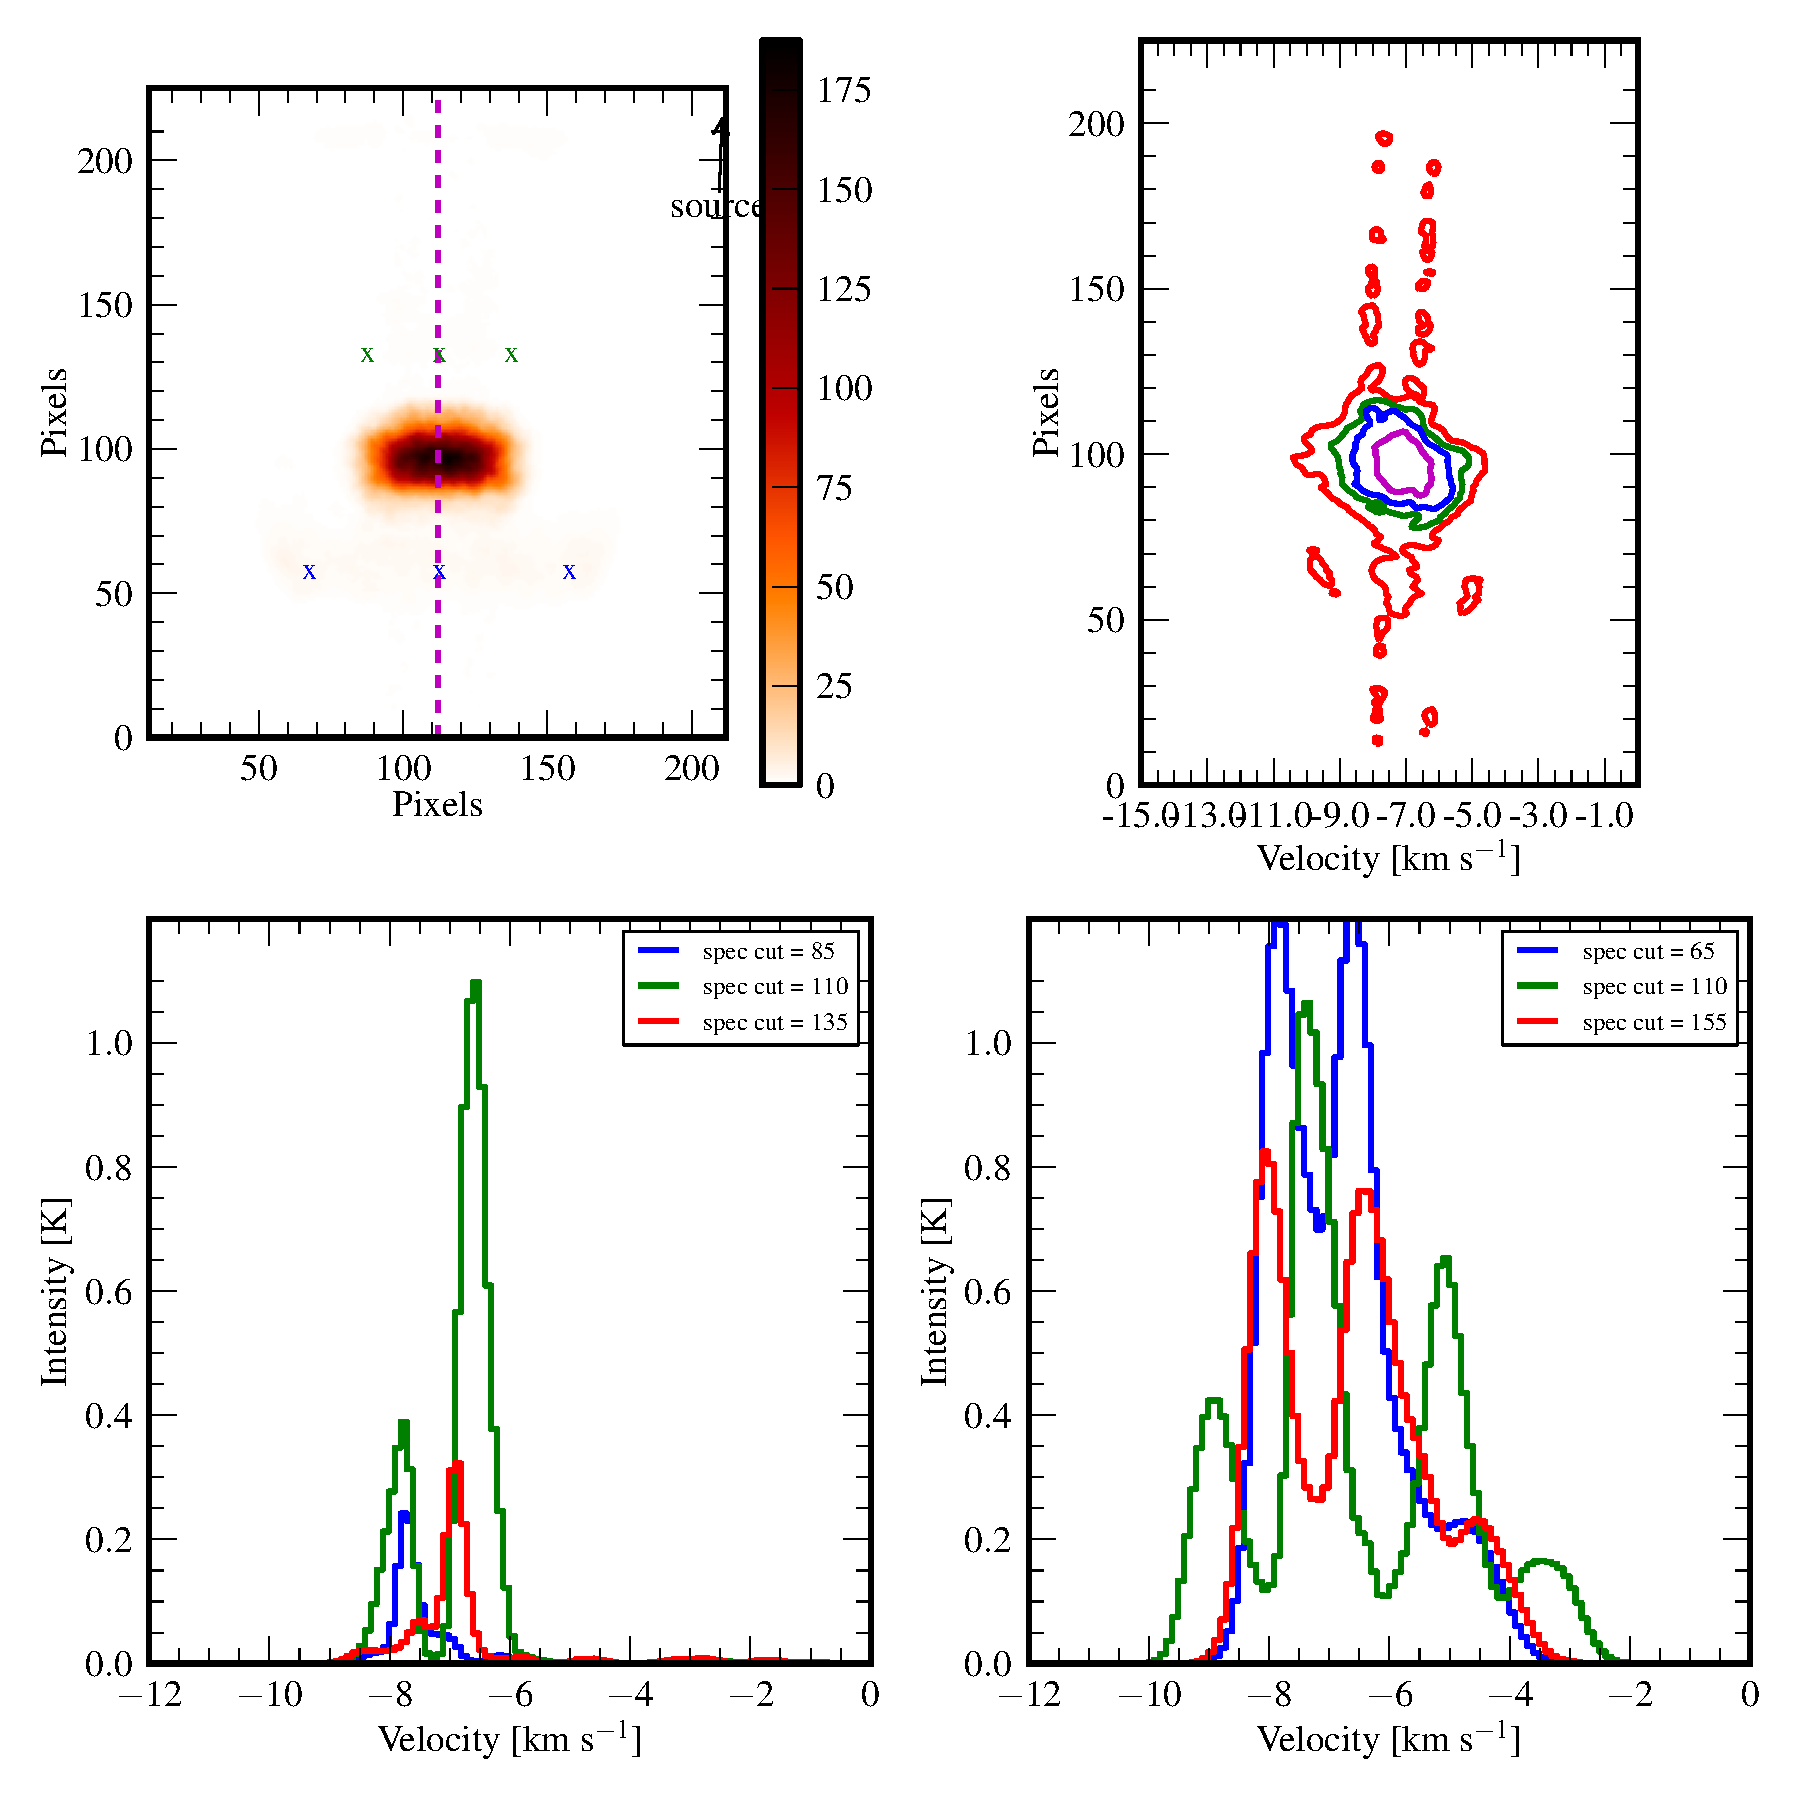
\includegraphics[scale=0.16]{knot_ang85.pdf} \\
\tiny{McCaughrean 2002} & \tiny{Codella 2007} & \tiny{Present work SiO(8-7)}\\
\end{tabular}
\end{frame}

\begin{frame}[T]
\frametitle{3D Modelling of Young Stellar Jets}
Re-collimation shocks and wiggles!
\animategraphics[autoplay,loop,scale=0.23]{2}{ImgJet3d/contourjet1.}{0000}{0060}
\end{frame}
\end{document}

